
\section{\label{sec:tutorial:shearwave:tet4}3D Bar Discretized with Tetrahedra}

PyLith features discussed in this tutorial:
\begin{itemize}
\item Dynamic solution
\item LaGriT mesh format
\item Absorbing dampers boundary conditions
\item Kinematic fault interface conditions
\item Elastic isotropic linearly elastic material
\item VTK output
\item Linear tetrahedral cells
\item SimpleDB spatial database
\item ZeroDispDB spatial database
\end{itemize}
All of the files necessary to run the examples are contained in the
directory \texttt{examples/bar\_shearwave/tet4.}


\subsection{Mesh Generation}

The mesh is a simple rectangular prism 8 km by 400 m by 400m (Figure
\ref{fig:shearwave:tet4:mesh}). This mesh could be generated via
a simple script, but it is even easier to generate this mesh using
LaGriT. We provide documented LaGriT files in \texttt{examples/bar\_shearwave/tet4.}
We first create the geometry and regions, mesh the domain using tetrahedral
cells, and then create point sets associated with boundary conditions.

\noindent \begin{center}
\begin{figure}
\begin{centering}
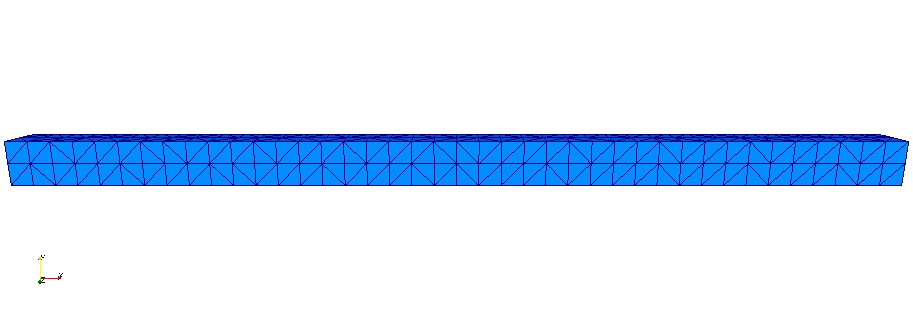
\includegraphics[scale=0.5]{tutorials/shearwave/figs/tet4mesh}
\par\end{centering}

\caption{Mesh composed of tetrahedral cells generated by LaGriT used for the
example problem.\label{fig:shearwave:tet4:mesh}}
\end{figure}

\par\end{center}


\subsection{Simulation Parameters}

The simulation parameters match those in the tri3 example with the
exception of using the LaGriT mesh reader and switching from a two-dimensional
problem to a three-dimensional problem. In addition to fixing the
longitudinal degree of freedom, we also fix the out-of-plane transverse
degree of freedom. Because the fault separates two material regions
in LaGriT, we use two materials in PyLith. All of the parameters are
set in the \texttt{pylithapp.cfg} file. To run the problem, simply
run PyLith without any command line arguments:
\begin{lyxcode}
pylith
\end{lyxcode}
The VTK files will be written to the \texttt{output} directory. The
output includes the displacement and velocity fields over the entire
domain at every 3rd time step (0.10 s), the slip and change in traction
vectors on the fault surface in along-strike and normal directions
at every 3rd time step (0.10 s), and the strain and stress tensors
for each cell at every 30th time step (1.0 s). If the problem ran
correctly, you should be able to generate a figure such as Figure
\ref{fig:shearwave:tet4:deform}, which was generated using ParaView.

\noindent \begin{center}
\begin{figure}
\begin{centering}
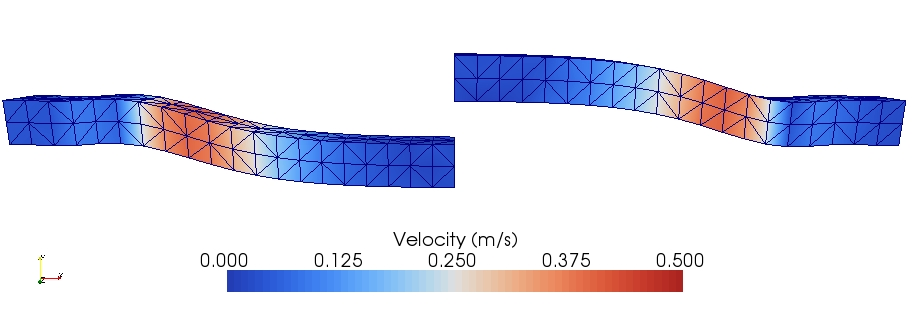
\includegraphics[scale=0.5]{tutorials/shearwave/figs/tet4deform30}
\par\end{centering}

\caption{Displacement field in the bar at 3.0 s. Deformation has been exaggerated
by a factor of 800.\label{fig:shearwave:tet4:deform}}
\end{figure}

\par\end{center}
